%%%%%%%%%%%%%%%%%%%%%%%%%%%%%%%%%%%%%%%%%
% Beamer Presentation
% LaTeX Template
% Version 1.0 (10/11/12)
%
% This template has been downloaded from:
% http://www.LaTeXTemplates.com
%
% License:
% CC BY-NC-SA 3.0 (http://creativecommons.org/licenses/by-nc-sa/3.0/)
%
%%%%%%%%%%%%%%%%%%%%%%%%%%%%%%%%%%%%%%%%%

%----------------------------------------------------------------------------------------
%	PACKAGES AND THEMES
%----------------------------------------------------------------------------------------

\documentclass{beamer}

\mode<presentation> {

% The Beamer class comes with a number of default slide themes
% which change the colors and layouts of slides. Below this is a list
% of all the themes, uncomment each in turn to see what they look like.

%\usetheme{default}
%\usetheme{AnnArbor}
%\usetheme{Antibes}
%\usetheme{Bergen}
%\usetheme{Berkeley}
%\usetheme{Berlin}
%\usetheme{Boadilla}
\usetheme{CambridgeUS}
%\usetheme{Copenhagen}
%\usetheme{Darmstadt}
%\usetheme{Dresden}
%\usetheme{Frankfurt}
%\usetheme{Goettingen}
%\usetheme{Hannover}
%\usetheme{Ilmenau}
%\usetheme{JuanLesPins}
%\usetheme{Luebeck}
%\usetheme{Madrid}
%\usetheme{Malmoe}
%\usetheme{Marburg}
%\usetheme{Montpellier}
%\usetheme{PaloAlto}
%\usetheme{Pittsburgh}
%\usetheme{Rochester}
%\usetheme{Singapore}
%\usetheme{Szeged}
%\usetheme{Warsaw}

% As well as themes, the Beamer class has a number of color themes
% for any slide theme. Uncomment each of these in turn to see how it
% changes the colors of your current slide theme.

%\usecolortheme{albatross}
%\usecolortheme{beaver}
%\usecolortheme{beetle}
%\usecolortheme{crane}
\usecolortheme{dolphin}
%\usecolortheme{dove}
%\usecolortheme{fly}
%\usecolortheme{lily}
%\usecolortheme{orchid}
%\usecolortheme{rose}
%\usecolortheme{seagull}
%\usecolortheme{seahorse}
%\usecolortheme{whale}
%\usecolortheme{wolverine}

%\setbeamertemplate{footline} % To remove the footer line in all slides uncomment this line
%\setbeamertemplate{footline}[page number] % To replace the footer line in all slides with a simple slide count uncomment this line

%\setbeamertemplate{navigation symbols}{} % To remove the navigation symbols from the bottom of all slides uncomment this line
}

\usepackage{graphicx} % Allows including images
\usepackage{booktabs} % Allows the use of \toprule, \midrule and \bottomrule in tables

%----------------------------------------------------------------------------------------
%	TITLE PAGE
%----------------------------------------------------------------------------------------

\title[VE216]{VE216 Recitation Class 2} % The short title appears at the bottom of every slide, the full title is only on the title page

\author{ZHU Yilun} % Your name
\institute[SJTU] % Your institution as it will appear on the bottom of every slide, may be shorthand to save space
{
UM-SJTU Joint Institute \\ % Your institution for the title page
\medskip
\textit{VE216 SU20 Teaching Group} % Your email address
}
\date{2020 Summer} % Date, can be changed to a custom date e.g.:\today

\begin{document}

\begin{frame}
\titlepage % Print the title page as the first slide
\end{frame}

\begin{frame}
\frametitle{Overview} % Table of contents slide, comment this block out to remove it
\tableofcontents % Throughout your presentation, if you choose to use \section{} and \subsection{} commands, these will automatically be printed on this slide as an overview of your presentation
\end{frame}

%----------------------------------------------------------------------------------------
%	PRESENTATION SLIDES
%----------------------------------------------------------------------------------------

%------------------------------------------------





%------------------------------------------------
\section{Chapter 1: Signals and Systems}
%------------------------------------------------






%-------------------------------------------------
\subsection{Properties of Systems}

\begin{frame}
    \frametitle{Systems}
\begin{itemize}
    \item Transform the input signal to the output signal
    \item Transformation is more general than function composition (which is pointwise)
    \bigskip
    \item invertible system vs. bijective (ve203)
    
    \item Understand the system in terms of input-output relation
    \item const. system $y(t) = 0$ vs. ``future'' $ y(t) = x(t+1) - x(t+1)$?
\end{itemize}

\end{frame}


\begin{frame}
\frametitle{Amplitude properties}
\begin{itemize}
\item linearity: zero in $\rightarrow$ zero out 
\begin{itemize}
    \item $ x(t) = 0,  \forall t$
    \item $y(t) = 2x(t) +1$
\end{itemize}
\bigskip
\item stability: bounded in $\rightarrow$ bounded out
\begin{itemize}
    \item should assume $x(t)$ bounded
    \item $y(t) = \int_{-\infty}^{t} x (\tau) d \tau$
\end{itemize}
\bigskip
\item invertibility: each output signal correspond to only one input signal 
\begin{itemize}
    \item $y(t)=x^2(t)$
\end{itemize}
 
\end{itemize}
\end{frame}
%-------------------------------------------------

\begin{frame}[t]
    \frametitle{Time properties: if no given formula}
    \begin{itemize}
        \item causality: output depends only on the ``present'' or ``past'' inputs
        \item time invariant: if $x(t) \rightarrow y(t)$, then $x(t-t_0) \rightarrow y(t-t_0)$
    \end{itemize}

    \begin{figure}
        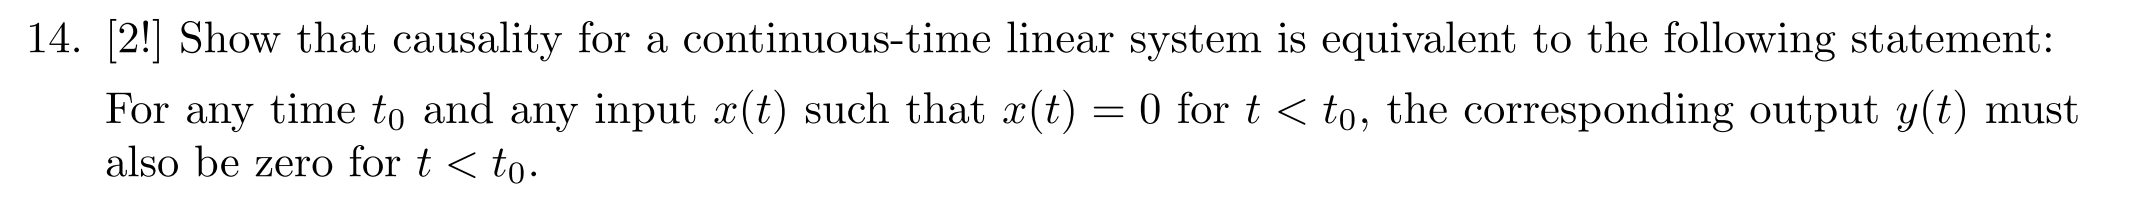
\includegraphics[width = 1\linewidth]{hw1_q14.PNG}
    \end{figure}

\end{frame}


\begin{frame}
    \frametitle{Exercise: Type 1 - Given Input-Ouput Pairs}
    \begin{block}{ Different from HW1 Q11}
    \begin{figure}
    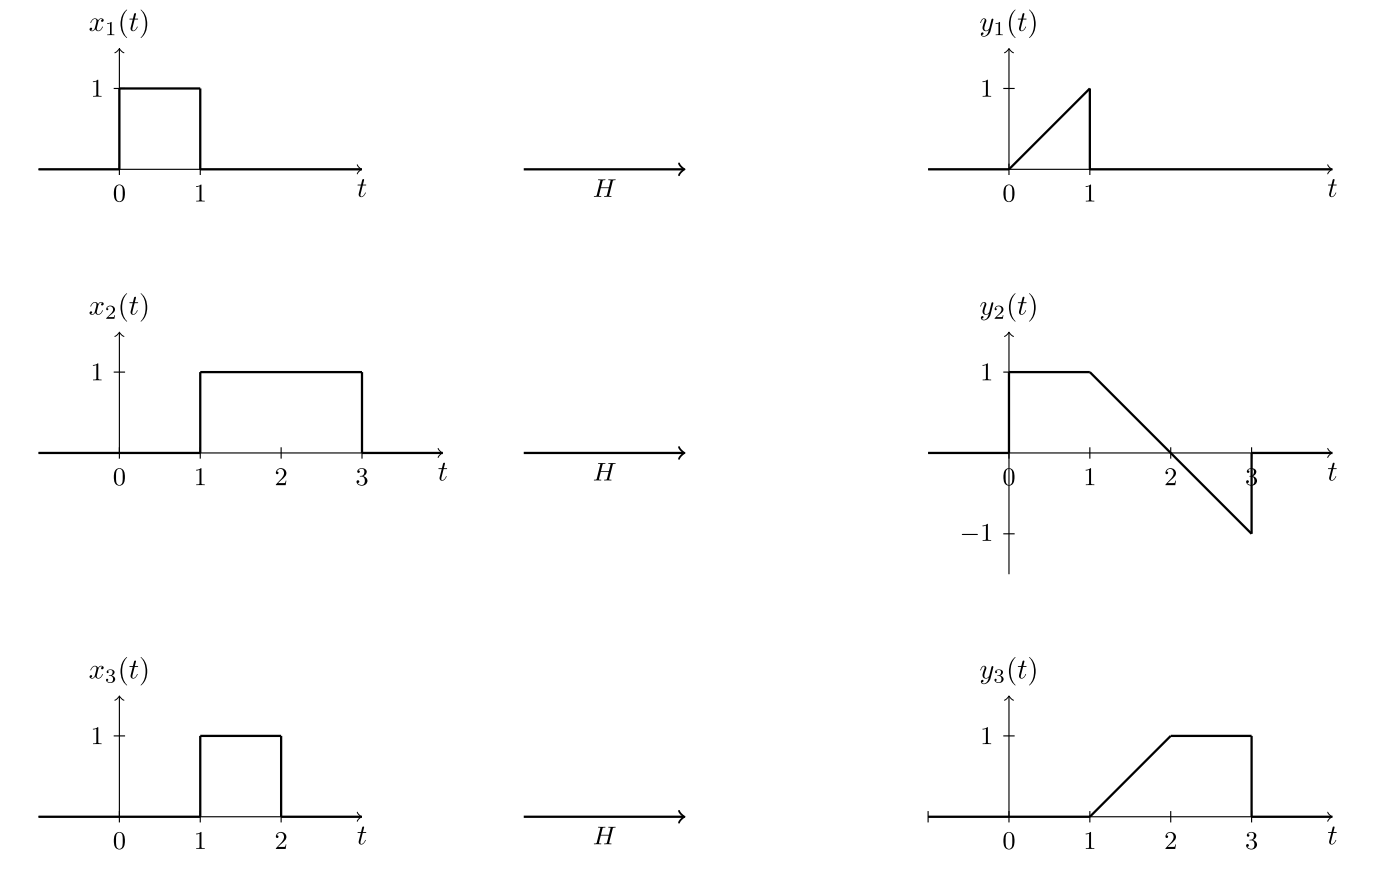
\includegraphics[width=0.6\linewidth]{hw1_q11}
    \end{figure}
    \end{block}
    \begin{itemize}
        \item Is it casual?
        \item Is it linear?
        \item If linear, is there other ways to determine casuality?    
    \end{itemize}
    
    \end{frame}
    
    \begin{frame}[t]
    \frametitle{Exercise}
    \begin{block}{Conti.}
    \begin{itemize}
    \item If linear, what is the output of $x_4(t)$ ?
    \begin{figure}
    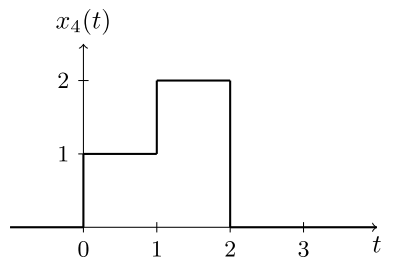
\includegraphics[width=0.4\linewidth]{exercise3}
    \end{figure}
    \end{itemize}
    \end{block}
\end{frame}


\begin{frame}[t]
\frametitle{Time properties}
\begin{itemize}
\item causality: output depends only on the ``present'' or ``past'' inputs
\item memoryless: output depends only on the ``present'' input $x(t)$
\item time invariant: if $x(t) \rightarrow y(t)$, then $x(t-t_0) \rightarrow y(t-t_0)$
\item Notice that the input refers to ``$x(t)$'', while there can be other terms relating to ``$t$'' 
\end{itemize}
Consider:
\[ y(t) = \frac{e^{x(t)}}{|t+1|} \]
\begin{itemize}
    \item casual:
    \item memoryless:
    \item Time Invariant:
\end{itemize}
\end{frame}

\subsection{Transformation of Signals}

\begin{frame}[t]
\frametitle{Transformation of Signals}
\begin{theorem}[Time transformation]
$1) \quad x(\frac{t-t_0}{w}) \qquad 2) \quad x(at-b)$
\end{theorem}
For Graph: \\
1) First scale according to $w$, then shift according to $t_0$ \\
2) First time-delay by $b$, then time-scale by $a$ 
\newline \\
Think about the physical meaning: 
There are two systems, one can shift the time, another can scale the time. Different sequence of connection requires different specification of ($w, t_0, a, b$) to reach the same effect. 
\newline 
\\
\bigskip
Question: for what system, the order doesn't matter?
\end{frame}

\begin{frame}
    \frametitle{Transformation of Signals}
    \begin{theorem}[Amplitude transformation]
    1) Reversal $y(t) = -x(t) $ \\
    2) Scaling $y(t) = ax(t)$ \\
    3) Shifting $y(t) = x(t) + b $\\
    \end{theorem}  
\end{frame}
    
\begin{frame}
    \frametitle{General Transformation}
    \begin{itemize}
    \item ``Time'' transformation: $ y(t) = x(g(t)) $ \\
    \item ``Amplitude'' transformation: $ y(t) = h(x(t)) $ \\
    \end{itemize}
Consider:
    \begin{itemize}
    \item 1) $y(t) = x(t) $
    \item  2) $y(t) = x(\sin(t))$   
    \item  3) $y(t) = \cos(x(t))$ 
    \item 4) $y(t)=\int_{-\infty}^{t/2}x(\tau)d\tau$               
    \end{itemize}
Question: \\
    \quad Think about whether the system that perform such transformation are: \\
    \quad ``linear, stable; time-invariant, causal, memoryless'' in general.  \\

\end{frame}


%-------------------------------------------------

\begin{frame}
\frametitle{Exercise: Type 2 - Given Formula}
General Transform - Revisited
\begin{itemize}
    \item ``Time'' transformation: $ y(t) = x(g(t)) $ \newline --- often lead to the violation of Time properties (TI, Casual)\\
    \item ``Amplitude'' transformation: $ y(t) = h(x(t)) $ 
    \newline --- often lead to the violation of Amplitude properties (linear)\\
    \end{itemize}
\begin{block}{Guess the result}

\begin{table}
\begin{tabular}{l l l l l l }
\toprule
\textbf{System} & \textbf{Time-Invariant Casual Linear Stable} \\
\midrule
$y(t) = x(2 - t)$ & \\
$y(t) = x(t/3)$ & \\
$y(t) = \int_{-\infty}^{t/2}x(\tau)d\tau$ & \\
$y(t) = cos(x(t))$ & \\

\bottomrule
\end{tabular}
%\caption{RC Arrangement}
\end{table}

\end{block}
\end{frame}



%------------------------------------------------
\section{Summary}
\begin{frame}
    \frametitle{Summary}
    \begin{itemize}
        \item Maybe you were confused about so many concepts and feel boring. 
        \item But at least I hope you could tell signal properties from system properties
        \item I would be glad if you can see the connection between signals and systems
        \item The first fascinating result: impulse response will be covered next week.
       
    \end{itemize}
    
\end{frame}

%------------------------------------------------

\begin{frame}
\Huge{\centerline{The End}}
%\huge{\centerline{See you next Thursday}}
\end{frame}

%----------------------------------------------------------------------------------------

\end{document} 